\documentclass{article}
\usepackage[utf8]{inputenc}
\usepackage{blindtext}
\usepackage[a4paper, total={6in, 10in}]{geometry}
\usepackage{tikz}
\usepackage{amsmath,amssymb}
\usepackage{mathptmx}
\usetikzlibrary{shapes.geometric}
\usepackage[nomessages]{fp}% http://ctan.org/pkg/fp
\usepackage[rightcaption]{sidecap}
\definecolor{B}{HTML}{2E79B2}
\definecolor{W}{HTML}{FF0000}


\begin{document}

\newcommand{\drawGraph}[1]{
\draw[step=1cm,gray,very thin] (-3,-3) grid (2,3);
\foreach \x in {-2,-1,0,1,2}
   \draw (\x cm,1pt) -- (\x cm,-1pt) node[anchor=north] {$\x$};
\foreach \y in {-2,-1,0,1,2}
    \draw (1pt,\y cm) -- (-1pt,\y cm) node[anchor=east] {$\y$};  
}

\newcommand{\drawGraphNo}[1]{
\draw [color=black](-3,0) -- (3,0);
\draw [color=black](0,-2) -- (0,3);
}
\newcommand{\labelForthree}[3]{
\tikzstyle{every node}=[draw];
%\node (v0) at (0:0) {$v_0$};
\node[top color=white] (v1) at (0:1.3){$#2$} ;
\node[top color=white] (v2) at (90:2) {$#3$};
\node[top color=white] (v3) at (2*90:1.2) {$#1$};
}

\newcommand{\drawTriangle}[3]{
\begin{tikzpicture}
    \drawGraphNo{3}
    \node[regular polygon,
    draw,minimum size=2cm,
    right color=white,left color=white,
    regular polygon sides = 3] (p) at (0,0.5){};
   \labelForthree{#1}{#2}{#3}
\end{tikzpicture}
}

\newcommand{\drawTrianglel}[7]{
\begin{tikzpicture}
    \drawGraphNo{3}
    \node[regular polygon,
    draw,minimum size=2cm,
    right color=white,left color=white,
    regular polygon sides = 3] (p) at (0,0.5){};
    \draw [dashed,color=black](#4,#5) -- (#6,#7);
   \labelForthree{#1}{#2}{#3}
\end{tikzpicture}
}

\section{\Large{Project 1}}

\large{QUESTIONS}
\begin{enumerate}
    \item construct Dihedral group $D_3$ and $D_5$
    \item Give two-dimensional representation of $D_3$ and $D5$
    \item let us have your creative pattern with polygon
    \item let us have  creative pattern with symmetric from nature
\end{enumerate}
\newcommand{\ArrowName}[1]{
\begin{tikzpicture}
    \draw [color=white](0,-3) -- (0,3);
    \draw [color=white](-2,0) -- (2,0);
    \draw[ultra thick, ->](-1,0) -- (1,0);
    \node at (0,0.3) {$#1$};
\end{tikzpicture}
}

\large{SOLUTIONS}
\subsection{Dihedral group of $D_3$ and $D_5$}
\Large{Dihedral group of  $D_3$}\\
r is a rotation through $360/n$\\
r= 360/3 = 120

Therefore we are rotating through 120.

$e=r_0$, rotation through $\theta=0$

\begin{enumerate}

\item{$r_0$:Rotation to angle $0^0$ anticlockwise }

\drawTriangle{1}{2}{3}
\ArrowName{r_0}
\drawTriangle{1}{2}{3}


\item{$r_1$: Rotation to angle $120^0$ anticlockwise }

\drawTriangle{1}{2}{3}
\ArrowName{r_1}
\drawTriangle{3}{1}{2}
\vspace{7cm}
\item{$r_2$:Rotation to angle $240^0$ anticlockwise }

\drawTriangle{1}{2}{3}
\ArrowName{r_2}
\drawTriangle{2}{3}{1}

\item{$f_1$:Reflection on y-axis }

\drawTrianglel{1}{2}{3}{0}{-2}{0}{2}
\ArrowName{f_1}
\drawTriangle{2}{1}{3}

\item{$f_2$: Reflection along vertex ($1$) and midpoint of  (2) and (3)}

\drawTrianglel{1}{2}{3}{2}{-0.6}{-2}{1.7}
\ArrowName{f_2}
\drawTriangle{3}{2}{1}
\vspace{4cm}
\item{$f_3$:Reflection along vertex ($3$) and midpoint of  (2) and (1)}

\drawTrianglel{1}{2}{3}{-2}{-0.6}{2}{1.7}
\ArrowName{f_3}
\drawTriangle{1}{3}{2}
\end{enumerate}
Therefore, $D_3=\{e,r,r^2,f_1,f_2,f_3\}$.

But, we can represent $f_1,f_2$ and $f_3$ in terms of f and r.

let $f_1$= f

then,

\newcommand{\NewOne}[3]{
\begin{tikzpicture}
\draw [color=black](-2,0) -- (2,0);
\draw [color=black](0,-1.7) -- (0,3);
    \node[regular polygon,
    draw,minimum size=2cm,
    right color=white,left color=white,
    regular polygon sides = 3] (p) at (0,0.5){};
   \labelForthree{#1}{#2}{#3}
\end{tikzpicture}}
\newcommand{\arrowP}[1]{
\begin{tikzpicture}
    \draw [color=white](0,-3) -- (0,3);
    \draw [color=white](-0.4,0) -- (0.4,0);
    \draw[ultra thick, ->](-0.4,0) -- (0.4,0);
    \node at (0,0.3) {$#1$};
\end{tikzpicture}}

\newcommand{\MidText}[1]{
\begin{tikzpicture}
    \draw [color=white](0,-3) -- (0,3);
    \draw [color=white](-0.4,0) -- (0.4,0);
    \draw[color=white](-0.4,0) -- (0.4,0);
    \node at (0,0.3) {$#1$};
\end{tikzpicture}}



\NewOne{1}{2}{3}
\arrowP{f}
\NewOne{2}{1}{3}
\arrowP{r}
\NewOne{3}{2}{1}
so,  rf=$f_3$

\NewOne{1}{2}{3}
\arrowP{f}
\NewOne{2}{1}{3}
\arrowP{r^2}
\NewOne{1}{3}{2}
so, $f_2=r^2f$

Now, we can have our $D_3$ to be:\\
 $D_3=$\{ $e,r,r^2,f,rf,r^2f$\}
 \vspace{2cm}

The Cayleys table below shows that $D_3$ is a group.\\
\begin{tabular}{| l | l | l | l |l |l |l |}
    $\circ$  & e & r& $r^2$& f &rf & $r^2f$ \\ 
    \hline
    e  & e & r& $r^2$& f &rf & $r^2f$ \\
     \hline
    r & r& $r^2$& e & rf & $r^2f$&f \\
    \hline
    $r^2$ &$r^2$ & e& $r$&$r^2f$  &f & $rf$ \\
    \hline
    f &f& $r^2f$& rf& e & $r^2$ & $r$ \\
     \hline
    rf & rf& f & $r^2f$ & r &e& $r^2$ \\
     \hline
    $r^2f$ &$r^2f$&rf &f& $r^2$ & r& e \\
    \hline
    \end{tabular}

\begin{itemize}
    \item Clearly $D_3$ equipped with composition is closed.
    \item the composition of function is known to be associative .
    \item every element n $D_3$ has an inverse 
\item e is the identity element 
\end{itemize}

\pmb{Therefore $D_3$ is a group.}\\\\
\large{The matrices below give a two-dimensional representation of $D_3$ }\\

For $r_0 \in D_3$ , $\theta = 0$\\

$\phi(r_0) =  $ 
$\begin{pmatrix}
    cos 0 & -sin 0\\
    sin 0 & cos 0
\end{pmatrix}$=$\begin{pmatrix}
    1& 0\\
    0 & 1
\end{pmatrix}$\\

For $r_{120^0} \in D_3$ , $\theta = 120^0$\\

$\phi(r_{120}) =  $ 
$\begin{pmatrix}
    cos 120 & -sin 120\\
    sin 120 & cos 120
\end{pmatrix}$=
$\begin{pmatrix}
   - \frac{1}{2}& -\frac{\sqrt{3}}{2}\\
    \frac{\sqrt{3}}{2} & - \frac{1}{2}
\end{pmatrix}$
\\

For $r_{240^0} \in D_3$ , $\theta = 240^0$\\

$\phi(r_{240}) =  $ 
$\begin{pmatrix}
    cos 240 & -sin 240\\
    sin 240 & cos 240
\end{pmatrix}$=
$\begin{pmatrix}
   - \frac{1}{2}& \frac{\sqrt{3}}{2}\\
    -\frac{\sqrt{3}}{2} & - \frac{1}{2}
\end{pmatrix}$
\\\\

REFECTION: using the general formula\\

$\begin{pmatrix}
    cos \frac{2\pi k}{n} & sin\frac{2\pi k}{n}\\
    sin \frac{2\pi k}{n} & -cos \frac{2\pi k}{n}
\end{pmatrix}$\\\\

When k=0, $\begin{pmatrix}
    1 & 0\\
    0 & 1
\end{pmatrix}$\\\\

When k=1, $\begin{pmatrix}
     - \frac{1}{2} & \frac{\sqrt{3}}{2}\\
    \frac{\sqrt{3}}{2}& \frac{1}{2}
\end{pmatrix}$\\\\

When k=2, 
$\begin{pmatrix}
     - \frac{1}{2} & -\frac{\sqrt{3}}{2}\\
    -\frac{\sqrt{3}}{2}& \frac{1}{2}
\end{pmatrix}$\\


\LARGE{DIHEDRA GROUP OF PENTAGON($D_5$)}
\newcommand{\pentagonDraw}[6]{
\begin{tikzpicture}
\drawGraphNo{3} 
\node (p) [draw,rotate=70,minimum size=3cm,regular polygon, regular polygon sides=#1] at (0,-0.4) {};
\tikzstyle{every node}=[draw,color=black];
\node[anchor=1*(360/9)]at(p.corner 1){$#2$};
\node[anchor=2*(360/9)]at(p.corner 2){$#6$};
\node[anchor=3*(360/9)]at(p.corner 3){$#5$};
\node[anchor=4*(360/9)]at(p.corner 4){$#4$};
\node[anchor=5*(360/9)]at(p.corner 5){$#3$};
\end{tikzpicture}
}

r is a anticlockwise rotation through $\frac{360^0}{n}=\frac{360}{5}=72^0$\\\\

\begin{enumerate}
\item e=$r_0$ (rotation through $\theta=0^0$)

\pentagonDraw{5}{5}{4}{3}{2}{1}
\ArrowName{e}
\pentagonDraw{5}{5}{4}{3}{2}{1}

\item{$r_{72^0}=r$ }\\
\pentagonDraw{5}{5}{4}{3}{2}{1}
\ArrowName{r}
\pentagonDraw{5}{4}{3}{2}{1}{5}
\item{$r_{144^0}=r^2$ }\\
\pentagonDraw{5}{5}{4}{3}{2}{1}
\ArrowName{r^2}
\pentagonDraw{5}{3}{2}{1}{5}{4}
\item{$r_{216^0}=r^3$ }\\
\pentagonDraw{5}{5}{4}{3}{2}{1}
\ArrowName{r^3}
\pentagonDraw{5}{2}{1}{5}{4}{3}

\item{$r_{288^0}=r^4$ }\\
\pentagonDraw{5}{5}{4}{3}{2}{1}
\ArrowName{r^4}
\pentagonDraw{5}{1}{5}{4}{3}{2}
\vspace{7cm}
\newcommand{\pentagonDrawl}[5]{
\drawGraphNo{3}
\node (p) [draw,rotate=70,minimum size=2.7cm,regular polygon, regular polygon sides=5] at (0,-0.4) {};
\tikzstyle{every node}=[draw,color=black];
\node[anchor=1*(360/9)]at(p.corner 1){$#1$};
\node[anchor=2*(360/9)]at(p.corner 2){$#5$};
\node[anchor=3*(360/9)]at(p.corner 3){$#4$};
\node[anchor=4*(360/9)]at(p.corner 4){$#3$};
\node[anchor=5*(360/9)]at(p.corner 5){$#2$};
}

\vspace{3cm}
\item{$f_1$: Reflection along y-axis }

\begin{tikzpicture}
\pentagonDrawl{5}{4}{3}{2}{1}
\draw [dashed,color=black](0,2) -- (0,-2);
\end{tikzpicture}
\ArrowName{f_1}
\pentagonDraw{5}{3}{4}{5}{1}{2}

\item{$f_2$: Reflection along vertex $3$ and midpoint of 1 and 5}

\begin{tikzpicture}
\pentagonDrawl{5}{4}{3}{2}{1}
\draw [dashed,color=black](2,0.3) -- (-2,-1.1);
\end{tikzpicture}
\ArrowName{f_2}
\pentagonDraw{5}{1}{2}{3}{4}{5}

\item{$f_3$: Reflection along vertex 2 and the mid point of 4 and 5}

\begin{tikzpicture}
\pentagonDrawl{5}{4}{3}{2}{1}
\draw [dashed,color=black](-1.1,1.2) -- (1.8,-3);
\end{tikzpicture}
\ArrowName{f_3}
\pentagonDraw{5}{4}{5}{1}{2}{3}
\vspace{3cm}
\item{$f_4$: Reflection along vertex 1 and the mid point of 4 and 3}

\begin{tikzpicture}
\pentagonDrawl{5}{4}{3}{2}{1}
\draw [dashed,color=black](1.1,1.2) -- (-1.8,-3);
\end{tikzpicture}
\ArrowName{f_4}
\pentagonDraw{5}{2}{3}{4}{5}{1}

\item{$f_5$: Reflection along vertex 5 and the mid point of 2 and 3}

\begin{tikzpicture}
\pentagonDrawl{5}{4}{3}{2}{1}
\draw [dashed,color=black](-2,0.3) -- (2,-1.1);
\end{tikzpicture}
\ArrowName{f_5}
\pentagonDraw{5}{5}{1}{2}{3}{4}
\end{enumerate}

Therefore,\\

$D_5=\{e,r,r^2,r^3,r^4,f_1,f_2,f_3,f_4\,f_5\}$\\

But we can represent $f_1,f_2,f_3,f_4$ and $f_5$ in terms of f and r.
Now, 
et $f_1=f$\\

\vspace{8cm}
\MidText{rf=}
\pentagonDraw{5}{5}{4}{3}{2}{1}
\arrowP{ f }
\pentagonDraw{5}{3}{4}{5}{1}{2}
\ArrowName{r}
\pentagonDraw{5}{4}{5}{1}{2}{3}
\MidText{=f_2}
\\\\


\MidText{r^2f=}
\pentagonDraw{5}{5}{4}{3}{2}{1}
\arrowP{ f }
\pentagonDraw{5}{3}{4}{5}{1}{2}
\ArrowName{r^2}
\pentagonDraw{5}{5}{1}{2}{3}{4}
\MidText{=f_3}\\

\MidText{r^3f=} 
\pentagonDraw{5}{5}{4}{3}{2}{1}
\arrowP{f}
\pentagonDraw{5}{3}{4}{5}{1}{2}
\ArrowName {r^3}
\pentagonDraw{5}{1}{2}{3}{4}{5} 
\MidText{=f_4}

\MidText{r^3f=} 
\pentagonDraw{5}{5}{4}{3}{2}{1}
\arrowP{f}
\pentagonDraw{5}{3}{4}{5}{1}{2}
\ArrowName {r^3}
\pentagonDraw{5}{3}{4}{5}{1}{2}
\MidText{=f_4}\\\\
Then, we can write $D_5$ as \\
$D_5=\{e,r,r^2,r^3,r^4,f,rf,r^2f,r^3f,r^4f\}$\\

The Cayleys table below shows that $D_3$ is a group.\\
\begin{tabular}{| l | l | l | l |l |l |l |l |l |l |l |}
\hline
$\circ$ & e &$ r $&$ r^2 $&$ r^3 $&$ r^4 $&$ f $&$ rf $&$ r^2f $&$ r^3f $&$ r^4f$ \\
\hline
e &$ e $&$ r $&$ r^2 $&$ r^3 $&$ r^4 $&$ f $&$ rf $&$ r^2f $&$ r^3f $&$ r^4f$ \\
\hline
r &$ r $&$ r^2 $&$ r^3 $&$ r^4 $&$ e $&$ rf $&$ r^2f $&$ r^3f $&$ r^4f $&$ f$ \\
\hline
$r^2$&$ r^2 $&$ r^3 $&$ r^4 $&$ e $&$ r $&$ r^2f $&$ r^3f $&$ r^4f $&$ f $& rf\\
\hline
$r^3$&$ r^3 $&$ r^4 $&$ e $&$ r $&$r^2$&$ r^2f $&$ r^3f $&$ r^4f $&$ f $& rf\\
\hline
$r^4$ &$ r^4 $&$ e $&$ r^2 $&$ r^3  $&$ r^4f $&$ f $& rf& rf &$ r^2f $&$ r^3f$\\
\hline
f &$ f $&$ r^4f $&$ r^3f $&$ r^2f  $&$ rf $&$ e $&$ r^4$&$ r^3 $&$ r^2 $& r\\
\hline
rf& rf &$ f $&$ r^4f $&$ r^3f $&$ r^2f $&$ r  $&$ e $&$ r^4 $&$ r^3 $&$  r^2$ \\
\hline
$r^2f$&$ r^2f $&$ rf $&$ f $&$ r^4f $&$ r^3f $&$ r^2 $&$ r  $&$ e $&$ r^4 $&$ r^3$
\\\hline
$r^3f$& $r^3f $&$r^2f $&$ rf $&$ f $&$ r^4 $&$ r^3 $&$ r^2 $&$ r  $&$ e $&$ r^4$ \\
\hline
$r^4$f& $r^4f$& $r^3f$&$r^2f $&$ rf $&$ f $&$ r^4 $&$ r^3 $&$ r^2 $&r &e\\
\hline
\end{tabular}
\\

\pmb{for $e=r_0 \in D_5, \theta =0^0$}\\
$\phi (r_0) = 
\begin{pmatrix}
cos 0^0 & -sin 0^0\\
sin 0^0 & cos0^0
\end{pmatrix} =
\begin{pmatrix}
1 & 0\\
0 & 1
\end{pmatrix} $\\\\
\vspace{4cm}

\pmb{for $r=r_{72^0} \in D_5, \theta =72^0$}\\
$\phi (r_{72^0}) = 
\begin{pmatrix}
cos 72^0 & -sin 72^0\\
sin 72^0 & cos72^0
\end{pmatrix} =
\begin{pmatrix}
\frac{-1+\sqrt(5)}{4} & \frac{-\sqrt(\frac{1}{2}*(5+\sqrt(5)))}{2}\\
\frac{\sqrt(\frac{1}{2}*(5+\sqrt(5)))}{2}& \frac{-1+\sqrt(5)}{4}
\end{pmatrix} $\\\\

\pmb{for $r^3=r_{144^0} \in D_5, \theta =144^0$}\\
$\phi (r_{144^0}) = 
\begin{pmatrix}
cos 144^0 & -sin 144^0\\
sin 144^0 & cos144^0
\end{pmatrix} =
\begin{pmatrix}
\frac{-1-\sqrt(5)}{4} & \frac{-\sqrt(\frac{1}{2}*(5+\sqrt(5)))}{2}\\
\frac{\sqrt(\frac{1}{2}*(5+\sqrt(5)))}{2}& \frac{-1-\sqrt(5)}{4}
\end{pmatrix} $\\\\

\pmb{for $r^3=r_{216^0} \in D_5, \theta =216^0$}\\
$\phi (r_{216^0}) = 
\begin{pmatrix}
cos 216^0 & -sin 216^0\\
sin 216^0 & cos216^0
\end{pmatrix} =
\begin{pmatrix}
\frac{-1-\sqrt(5)}{4} & \frac{\sqrt(\frac{1}{2}*(5+\sqrt(5)))}{2}\\
-\frac{\sqrt(\frac{1}{2}*(5+\sqrt(5)))}{2}& \frac{-1-\sqrt(5)}{4}
\end{pmatrix} $\\\\

\pmb{for $r^4=r_{288^0} \in D_5, \theta =288^0$}\\
$\phi (r_{288^0}) = 
\begin{pmatrix}
cos 288^0 & -sin 288^0\\
sin 288^0 & cos288^0
\end{pmatrix} =
\begin{pmatrix}
\frac{-1+\sqrt(5)}{4} & \frac{\sqrt(\frac{1}{2}*(5+\sqrt(5)))}{2}\\
-\frac{\sqrt(\frac{1}{2}*(5+\sqrt(5)))}{2}& \frac{-1+\sqrt(5)}{4}
\end{pmatrix} $\\\\



\pmb{REFLECTION}\\
Using the genera formuar;\\

$\begin{pmatrix}
cos \frac{2 \pi k}{n} & -sin \frac{2 \pi k}{n}\\
sin \frac{2 \pi k}{n} & cos\frac{2 \pi k}{n}
\end{pmatrix}$
where, n=5, k=0,1,2,3,4\\\\

when k=0,\\
$\begin{pmatrix}
1 & 0\\
0 & 1
\end{pmatrix}$\\

when k=1\\
$\begin{pmatrix}
\frac{-1+\sqrt(5)}{4} & \frac{\sqrt(\frac{1}{2}*(5+\sqrt(5)))}{2}\\
\frac{\sqrt(\frac{1}{2}*(5+\sqrt(5)))}{2}& \frac{1-\sqrt(5)}{4}
\end{pmatrix}$ \\


when k=2\\
$\begin{pmatrix}
\frac{-1-\sqrt(5)}{4} & \frac{\sqrt(\frac{1}{2}*(5-\sqrt(5)))}{2}\\
\frac{\sqrt(\frac{1}{2}*(5-\sqrt(5)))}{2}& \frac{1+\sqrt(5)}{4}
\end{pmatrix}$ \\

when k=3\\
$\begin{pmatrix}
\frac{-1-\sqrt(5)}{4} & -\frac{\sqrt(\frac{1}{2}*(5-\sqrt(5)))}{2}\\
-\frac{\sqrt(\frac{1}{2}*(5-\sqrt(5)))}{2}& \frac{1+\sqrt(5)}{4}
\end{pmatrix}$ 

when k=4\\
$\begin{pmatrix}
\frac{-1+\sqrt(5)}{4} & -\frac{\sqrt(\frac{1}{2}*(5-\sqrt(5)))}{2}\\
-\frac{\sqrt(\frac{1}{2}*(5+\sqrt(5)))}{2}& \frac{1-\sqrt(5)}{4}
\end{pmatrix}$ 
\\\\\\

\pmb{CREATIVE PATTERN WITH POLYGON}

\begin{enumerate}
    \item  Pattern with Square
\graphicspath{{pictures/}}
\begin{figure}[htp]
    \includegraphics[width=10cm]{create.jpg}
\end{figure}\\\\

\item Pentagon pattern
\begin{figure}[htp]
    \includegraphics[width=14cm]{create4.jpg}
\end{figure}
\end{enumerate}
\vspace{14cm}
\pmb{CREATIVE PATTERN FROM NATURE}

\begin{enumerate}
    \item Aloe polyphylla
\graphicspath{{pictures/}}
\begin{figure}[htp]
    \includegraphics[width=6cm]{nature1.jpg}
    \includegraphics[width=9cm]{nature2.jpg}
\end{figure}
\\
This is an  evergreen succulent perennial, it is well known for its strikingly symmetrical, pointed spiral growth habit. It is a stemless aloe and grows its leaves in a very distinctive spiral shape which may be clockwise or anti-clockwise. 
It is often grown as an ornamental plant in rock gardens, containers, or as a focal point in xeriscape landscapes. In addition to its ornamental value, Aloe polyphylla has been used in traditional medicine to treat a variety of ailments, including digestive issues and skin conditions.
\end{enumerate}
\section{Project 2}
\begin{enumerate}
    \item Describe the group of symmetry of a rectangle
    \item Describe the group of symmetry of a Cube and tetrahedron
   \item Describe square in dimension 3, 4, and 5
\end{enumerate}

\newcommand{\Rectang}[4]{
\begin{tikzpicture}
\drawGraphNo{3}
\draw (-2,1)[] -| node[pos=0,left]{$#1$} 
              node[pos=.5,right]{$#2$} 
              (2,-1) -|  node[pos=0,right]{$#3$}
  node[pos=.5,left]{$#4$} cycle;

\end{tikzpicture}
}
\\
\pmb{SOLUTION}\\
r is the rotation through 360/n\\
$r=360^0/4=90^0$\\
But a rectangle is an irregular shape. then, to get symmetry, we have to rate it through $180^0$.

\begin{enumerate}
\item{e: Rotation to angle $0^0$ anticlockwise}

\Rectang{4}{3}{2}{1}
\ArrowName{e}
\Rectang{4}{3}{2}{1}
\vspace{4cm}
\item{r: Rotation to angle $180^0$ anticlockwise}

\Rectang{4}{3}{2}{1}
\ArrowName{r}
\Rectang{2}{1}{4}{3}

\item{$f_0$: Refection through y-axis }

\Rectang{4}{3}{2}{1}
\ArrowName{f_0}
\Rectang{3}{4}{2}{1}

\item{$f_1$:Refection through x-axis  }

\Rectang{4}{3}{2}{1}
\ArrowName{f_1}
\Rectang{1}{2}{4}{3}
\end{enumerate}
\vspace{4cm}
The Cayleys table below shows that $D_2$ is a group.\\\\

\begin{tabular}{| l | l | l | l |l |}
\hline
$\circ$& e& r & f & rf \\
\hline
e& e& r & f & rf \\
\hline
r& r& e & rf & f\\ 
\hline
f& f& rf& e & r \\
\hline
rf& rf&f &r & e \\
\hline
\end{tabular}\\

From the table we deduced that ( $D_2$) is an abelian group\\\\

\pmb{Group of symmetry of a cube}\\\\
\begin{figure}[htp]
    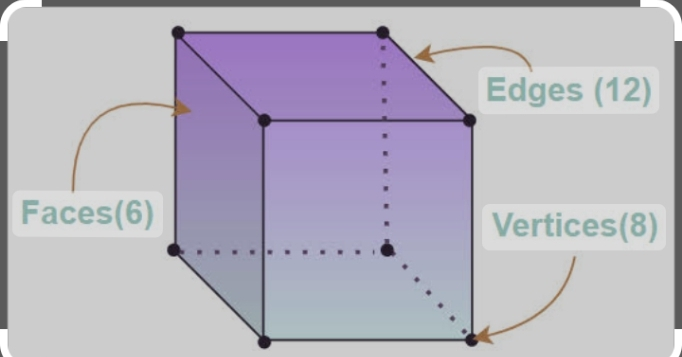
\includegraphics[width=9cm]{pictures/pict0.jpg}
\end{figure}\\
A symmetry of a cube is a permutation of its eight corners that sends edges to edges; in other words if a pair of corners are joined by an edge, then each symmetry must send this pair to another pair that is also joined by an edge. A cube has 48 symmetries, 24 of which can be realised physically  on a solid cube; the other 24 effectively turn the cube inside out. To see why there are 24 physical symmetries, notice that a cube has six faces any of which can be moved to the bottom, and this face can then be rotated into four different positions: 6* 4= 24.\\

Now, consider the 9 rotations of the cube about the 3 axes shown in the picture below.  We can either rotate by 90, 180 or 270 degrees around either the red, blue or green axes.  Each of these rotations will leave two faces fixed and all vertices and edges are not fixed.  When work out the cycle structure of these 9 elements notice that the 6 rotations by 90 or 270 degrees will have the same cycle structure and the 3 rotations of 180 degrees about each of the axes will have the same cycle structure.
\vspace{4cm}

\begin{figure}[htp]
    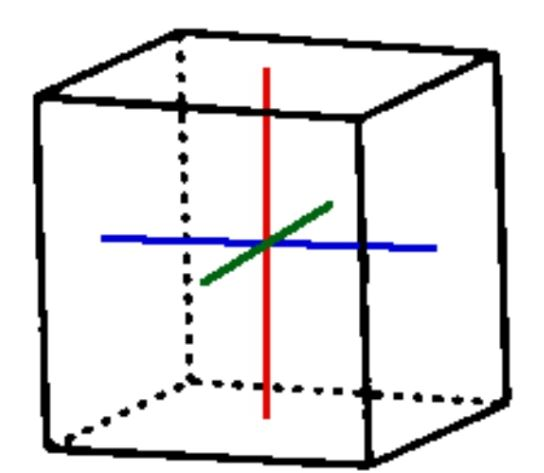
\includegraphics[width=6cm]{pictures/pict1.JPG}
\end{figure}


Next, consider the 6 rotations of the cube by 180 degrees around the 6 axes shown in the image below.  Each of these rotations leave two edges fixed and no faces or vertex Finally we have rotations by 120 and 240 degrees around the 4 axes shown in the image below.  This gives 8 permutations each of which leave 2 vertices fixed and no edges or faces fixed.  All 8 of these permutations will have the same cycle structure.
\\
\begin{figure}[htp]
    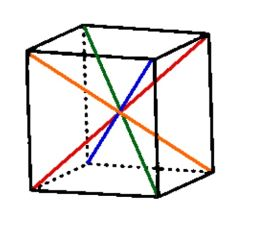
\includegraphics[width=6cm]{pictures/pict2.jpg}
\end{figure}

Finally we have rotations by 120 and 240 degrees around the 4 axes shown in the image below.  This gives 8 permutations each of which leave 2 vertices fixed and no edges or faces fixed.  All 8 of these permutations will have the same cycle structure.
\vspace{7cm}

\begin{figure}[htp]
    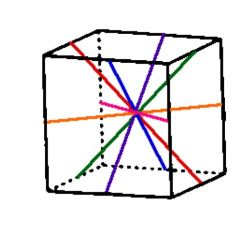
\includegraphics[width=7cm]{pictures/pict3.jpg}
\end{figure}\\

Since we have 1+9+6+8 = 24 permutations we need not look any further for others. We must have the whole group because, we already know that there were only 24\\
 \vspace{1cm}
 
\textbf{Reflection of a Cube}\\

\begin{figure}[htp]
    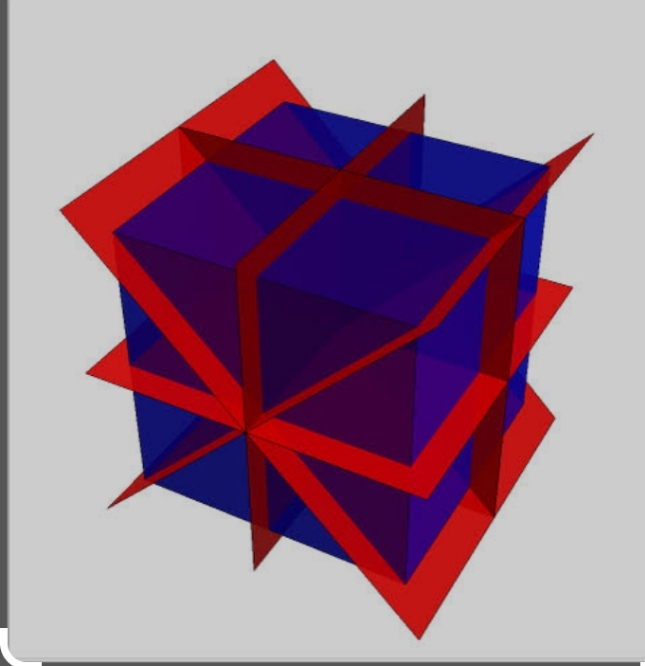
\includegraphics[width=10cm]{pictures/pict4.jpg}
\end{figure}\\

The symmetries of a cube of side length include two kinds of plane reflections.
There are 3 symmetries that are reflections in a plane parallel to a pair of faces of the cube. Each of these 3 planes intersects 4 edges at their midpoints; it is the perpendicular bisecting plane of 4 parallel edges.  The symmetry plane cuts the surface of the cube in a square of side s.  Each of the planes intersects 4 square faces. It intersects each face along a line of symmetry of the face that connects midpoints of opposite edges. Such a plane contains none of the vertices of the cube.The other 6 plane reflections are in planes that cut two opposite faces of cubes in diagonals.  Such a plane contains two opposite edges of the cube and 4 vertices.  Each such plane cuts the surface of the cube in a rectangle of width = s and length = s*sqrt 2.In the square figure above, if the square is a face of the cube, then two of the 3 planes of symmetry of the first type cut the square along the two lines of symmetry through the midpoints of the sides.  

Also, two of the 6 planes of symmetry of the second type cut the square along the lines of symmetry that are diagonals of the square.  Notice that the former lines are red and the diagonal lines are green. Compare this with the figure of a cube below.  The red segments represent the intersections of the 3 planes of symmetry of the first type with the 3 visible faces of the cube.  \\

The green dashed segments represent the intersections of the 6 planes of symmetry of the second type with the 3 visible faces of the cube.  Notice that each of these segments is along one of the lines of symmetry of a square face. Thus these planes cut each face of the cube into the same 8 congruent isosceles right triangles that were the fundamental regions of the symmetries of the square.  Since there are six faces, the surface of the cube is cut into 48 congruent isosceles right triangles.

\begin{figure}[htp]
    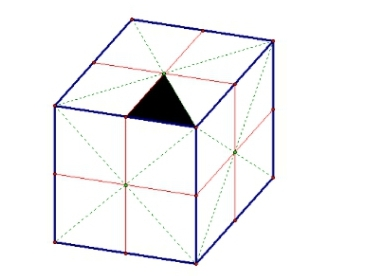
\includegraphics[width=10cm]{pictures/pictv.jpg}
\end{figure}
 \vspace{4cm}

\pmb{Symmetric of regular Tetrahedron}\\

\begin{figure}[htp]
\includegraphics[width=9cm]{pictures/prism00.jpg}
\end{figure}\\

There are 12 rotations of a tetrahedron shape. We can rotate through the vertices and through the edges. It is evident that rotating at 360°, we have; 
Rotating at vertex “1”. That is, rotating at 120°, we have:\\

 \begin{figure}[htp]
    \includegraphics[width=17cm]{pictures/prism1.jpg}
\end{figure}

\vspace{7cm}
  \begin{figure}[htp]
    \includegraphics[width=20cm]{prisim2.jpg}
\end{figure}
\vspace{7cm}
  \begin{figure}[htp]
    \includegraphics[width=18cm]{pictures/prism3.jpg}
\end{figure}

  \begin{figure}[htp]
    \includegraphics[width=17cm]{pictures/prism4.jpg}
\end{figure}

 \begin{figure}[htp]
    \includegraphics[width=17cm]{pictures/prismv.jpg}
\end{figure}\\

\\
First, note that a tetrahedron has four vertices. For each permutation of these vertices, there exists a symmetry in the total symmetry group. Specifically, the first vertex can take four different positions. The second vertex can then end up in any of the three remaining positions via rotation.The third vertex must then take any of the final two positions by reflection, and now the position of the fourth vertex remains fixed. \\
Therefore, under rotations and reflections, the Tetrahedron has 4 * 3 * 2 * 1 or 24 total symmetries. Observe that the order of S4, the Permutation Group of order 4, also has order 24. Now, each vertex can be labeled from 1 to 4, and thus, permutations of vertex positions can be expressed under cyclic notation. Using this notation, first the rotational symmetries can be listed out. A tetrahedron has two axes of symmetry, one passing through the center of one face and the vertex right above it, and another passing through the center of one edge and the perpendicular edge adjacent to it (Figure 1 below). We can label these axes of symmetry as L and M, respectively.\\

\begin{figure}[htp]
    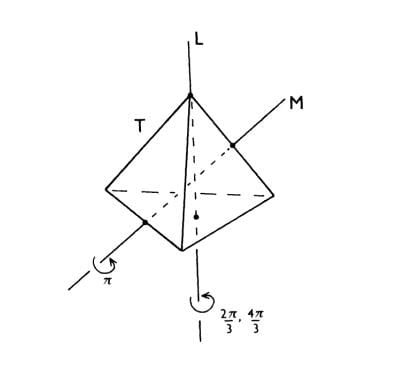
\includegraphics[width=10cm]{pictures/prism20.jpg}
    \caption{The axes of symmetry of the Tetrahedron.}
\end{figure}

Clearly, an axis of type L permutes only three vertices, and thus all three cycles of the vertex elements 1, 2, 3, and 4 describe rotations along such axes. Thus, the 8 possible three cycles (123), (132), (124), (142), (134), (143), (234), and (243) correspond to the possible 120 degree symmetry rotations. On the other hand, an axis of type M permutes all four vertices, swapping them in pairs. Thus, the three possible products of two disjoint transpositions, (12)(34), (13)(24), and (14)(23) correspond to elements of the rotational symmetries wherein the solid is revolving 180 degrees.The final rotational symmetry, the identity–not rotating the shape at all–corresponds to the cyclic notation describing no permutations, (). Note that these 12 possible rotational symmetries directly correspond to all even order elements of S4, otherwise known as the Alternating Group A4. Clearly when two rotations r and r' prompt permutations p and p' respectively, their composed rotation rr' prompts the permutation pp' , exhibiting a homomorphism. Moreover, the injective and surjective mapping explicitly listed out above exhibits a bijection. Thus, via this correspondence, the group of rotational symmetries of the Tetrahedron are isomorphic to A4.\\

On a similar note, the possible reflections of the tetrahedron can also be expressed using cyclic notation. Note that the only possible tetrahedral plane of symmetry would intersect both the midpoint of an edge and the opposite vertices of the two faces containing that edge. Equivalently, a plane of symmetry must be spanned by any two L and M axes of symmetry, and would swap any two vertices of the tetrahedron not contained in this plane. Thus all six transpositions of S4, (12), (13), (14), (23), (24), and (34), correspond to a reflectional symmetry. Now, the only elements that don’t correspond to a single reflection or rotation are remaining four cycles (1234), (1243), (1324), (1342), (1423), and (1432). We can see that (1234) is equivalent to the product (123)(34), and moreover, that the corresponding movement matches up with the composition of a reflection and rotation on the solid. Similarly all other elements of S4 can be mapped to by elements generated by rotations and reflections, and this map is thus surjective. Now, as all 24 elements of S4 map to the 24 possible rotation and reflection symmetries of the Tetrahedron, and compositions of these elements directly correspond on both sides of the mapping, the full group of symmetries is isomorphic to S4 \\
\begin{figure}[htp]
    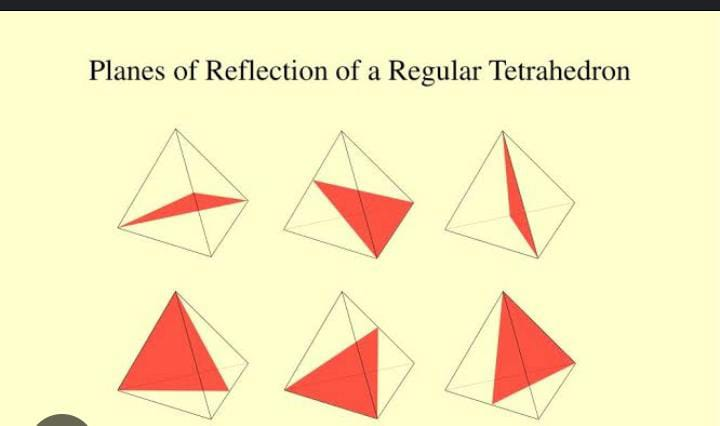
\includegraphics[width=17cm]{pictures/prismN.jpg}
\end{figure}\\
\vspace{11cm}

\pmb{Square in Differnt Dimension }\\\\
\begin{tabular}{| l | l | l |l |}
\hline
Name& 	Dimensions& 	Number of edges& 	Number of vertices\\
\hline
Square& 	2& 	4& 	4\\
\hline
Cube& 	3& 	12& 	8\\
\hline
Tesseract& 	4& 	32& 	16\\
\hline
Five-cube& 	5& 	80& 	32\\
\hline
\end{tabular}\\\\
The following shows the image of Square in dimension three, four and five\\
  \begin{figure}[htp]
    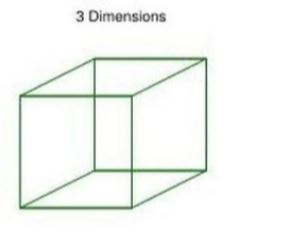
\includegraphics[width=7cm]{pictures/dimension3.jpg}
    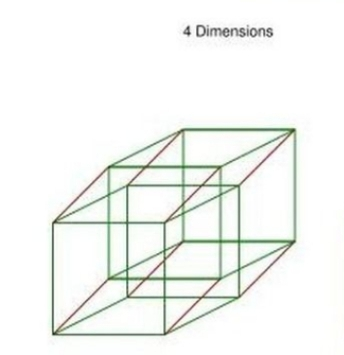
\includegraphics[width=7cm]{pictures/dimension4.jpg}
\end{figure}\\
 \begin{figure}[htp]
     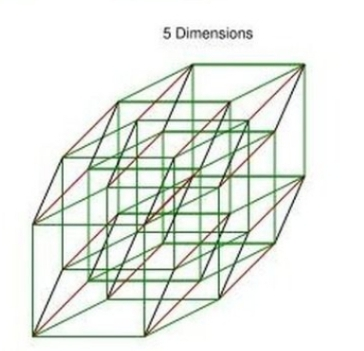
\includegraphics[width=6cm]{pictures/dimensionv.jpg}
\end{figure}
\end{document}
